\documentclass[tikz,border=5mm]{standalone}
\usepackage{tikz}
\usetikzlibrary{arrows.meta, positioning, shapes.geometric, calc, backgrounds, fit, matrix, patterns, decorations.pathmorphing, decorations.markings, shadows}

% --- COLOR DEFINITIONS ---
\definecolor{Garnet}{HTML}{73000A}
\definecolor{CSecondaryRed}{HTML}{CC2E40}
\definecolor{CBlue}{HTML}{466A9F}
\definecolor{CDark}{HTML}{1F414D}
\definecolor{COlive}{HTML}{65780B}
\definecolor{CLime}{HTML}{CED318}
\definecolor{CGold}{HTML}{A49137}
\definecolor{CGrayLight}{HTML}{E5E5E5}
\definecolor{CGrayDark}{HTML}{555555}
\definecolor{CWhite}{HTML}{FFFFFF}

\begin{document}

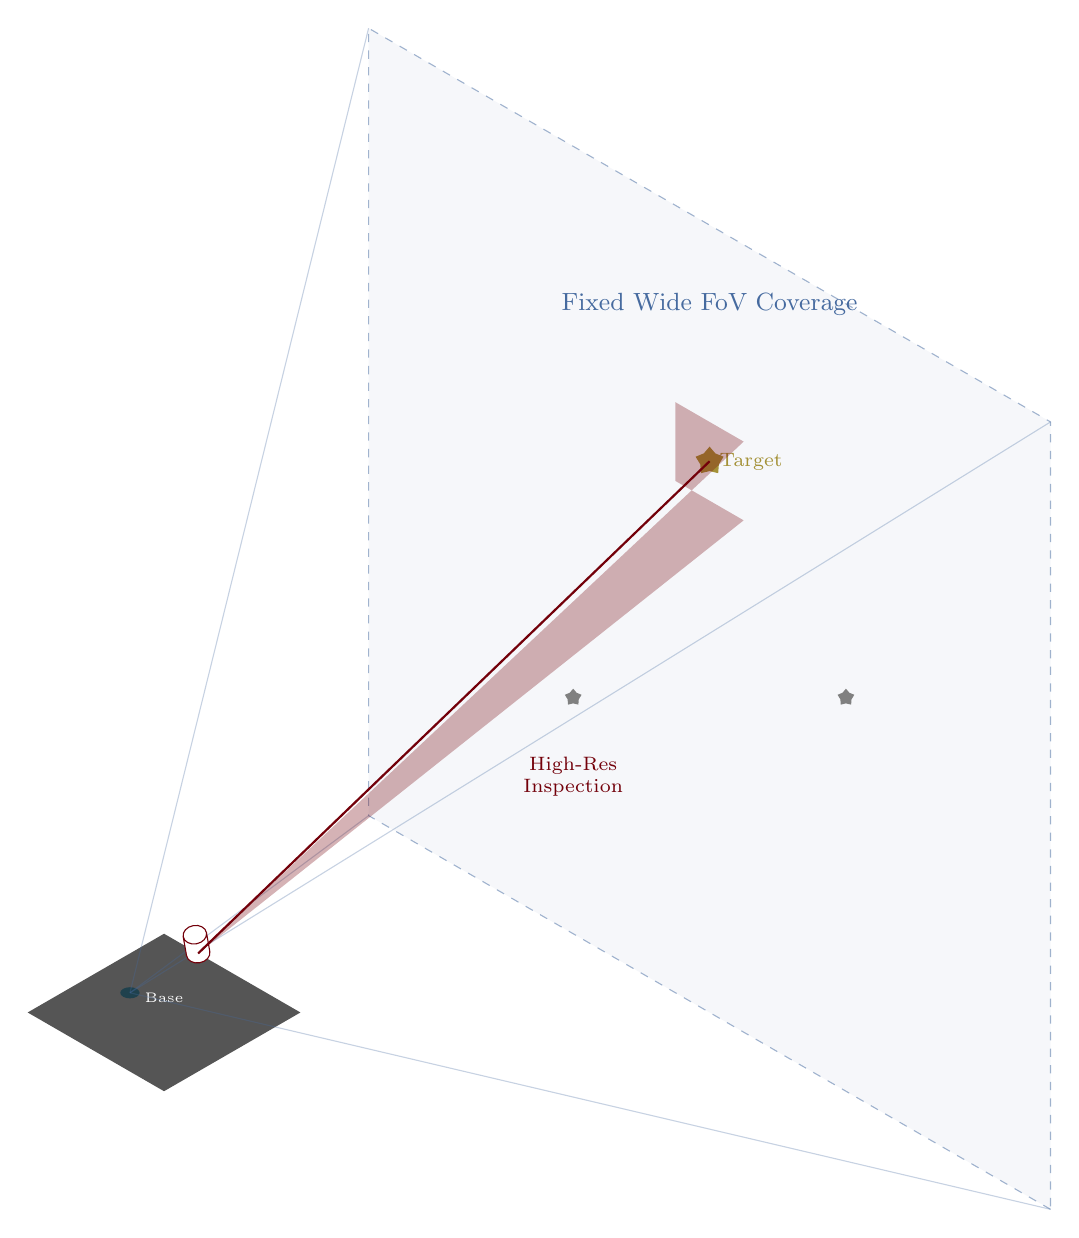
\begin{tikzpicture}[x={(0.866cm,0.5cm)}, y={(-0.866cm,0.5cm)}, z={(0cm,1cm)}]
    % Setup
    \coordinate (Origin) at (0,0,0);
    \coordinate (TargetPlaneDist) at (8,0,0); % Distance to target plane
    
    % Platform
    \fill[CGrayDark] (-1, -1, 0) -- (1, -1, 0) -- (1, 1, 0) -- (-1, 1, 0) -- cycle;
    \node[above, font=\tiny, white] at (0,0,0) {Base};

    % Targets in the distance
    % Let's define a virtual plane at x=8
    \coordinate (T1) at (8, -2, 1);
    \coordinate (T2) at (8, 0, 3);
    \coordinate (T3) at (8, 2, -1);
    
    % --- Wide Camera Coverage (The "Pyramid") ---
    % Originating roughly from center-left
    \coordinate (CamFixed) at (-0.5, 0, 0.5);
    \fill[CDark] (CamFixed) circle (0.1); 
    
    % Wide frustum corners at x=8
    \coordinate (BL) at (8, -5, -4);
    \coordinate (BR) at (8, 5, -4);
    \coordinate (TR) at (8, 5, 6);
    \coordinate (TL) at (8, -5, 6);
    
    % Draw Wide FoV Edges
    \draw[CBlue, thin, opacity=0.3] (CamFixed) -- (BL);
    \draw[CBlue, thin, opacity=0.3] (CamFixed) -- (BR);
    \draw[CBlue, thin, opacity=0.3] (CamFixed) -- (TR);
    \draw[CBlue, thin, opacity=0.3] (CamFixed) -- (TL);
    
    % Draw Wide FoV Face (The "Screen")
    \fill[CBlue, opacity=0.05] (BL) -- (BR) -- (TR) -- (TL) -- cycle;
    \draw[CBlue, dashed, opacity=0.5] (BL) -- (BR) -- (TR) -- (TL) -- cycle;
    \node[CBlue, font=\small] at (8, 0, 5) {Fixed Wide FoV Coverage};

    % --- Objects ---
    \foreach \p in {T1,T3} {
        \node[star, star points=5, fill=gray, inner sep=1.5pt] at (\p) {};
    }
    % Active Target
    \node[star, star points=5, fill=CGold, inner sep=2.5pt] (ActiveT) at (T2) {};
    \node[right, CGold, font=\scriptsize] at (T2) {Target};

    % --- PTZ Camera & Beam ---
    \coordinate (CamPTZ) at (0.5, 0, 0.5);
    \node[cylinder, draw=Garnet, fill=white, rotate=100, minimum height=0.4cm, minimum width=0.3cm] at (CamPTZ) {};
    
    % PTZ Beam (Narrow) pointing to T2
    % We create a small cone around T2
    \coordinate (P1) at ($(T2) + (0, -0.5, -0.5)$);
    \coordinate (P2) at ($(T2) + (0, 0.5, -0.5)$);
    \coordinate (P3) at ($(T2) + (0, 0.5, 0.5)$);
    \coordinate (P4) at ($(T2) + (0, -0.5, 0.5)$);
    
    \fill[Garnet, opacity=0.3] (CamPTZ) -- (P1) -- (P2) -- (P3) -- (P4) -- cycle;
    \draw[Garnet, thick] (CamPTZ) -- (T2);
    
    % Annotation
    \node[Garnet, align=center, font=\scriptsize] at (4, -2, 2) {High-Res\\Inspection};

\end{tikzpicture}

\end{document}
